\documentclass{article}
    \usepackage[utf8]{inputenc}
    \usepackage{natbib}
\usepackage{graphicx}
\usepackage{enumitem}
\usepackage{amsmath}
\usepackage{float}
\usepackage[a4paper]{geometry}
\usepackage[T1]{fontenc}
\usepackage{lipsum}
\usepackage{multicol}
\usepackage{changepage}



    \title{Assignment 2}
    \author{Yang Gao\\
        yanggao@kth.se}
    \date{May 2018}

    \usepackage{natbib}
    \usepackage{graphicx}

    \begin{document}

    \maketitle

    \section{Plot of Sound Signal Over Time Domain}
    The code used to generate following plot can be found in \texttt{plottime.m}]
    \\First, the music signal plot over time domain
    \begin{figure}[H]
        \begin{center}
        \leavevmode
        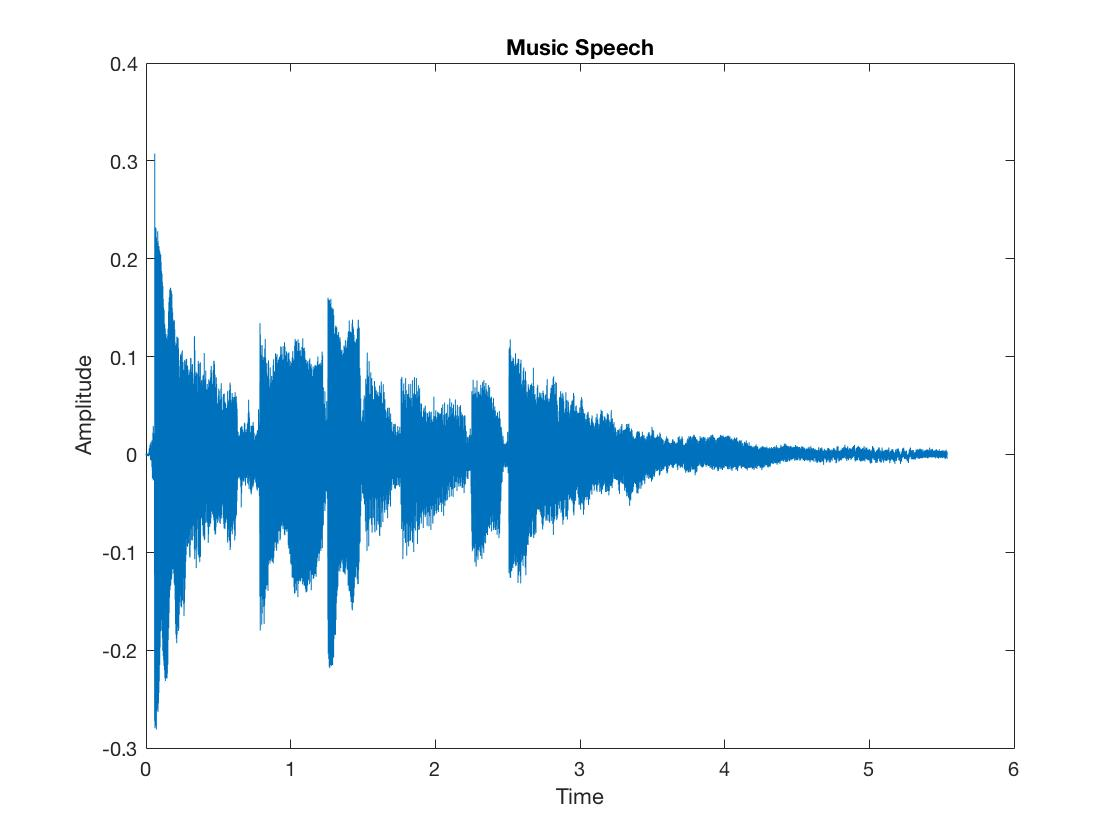
\includegraphics[width=0.75\textwidth]{music_time.jpg}
        \end{center}
        \caption{Music signal plot over time}
        \label{euler:1}
    \end{figure}
    \newpage
    Second, the female signal plot over the time domain
    \begin{figure}[H]
        \begin{center}
            \leavevmode
            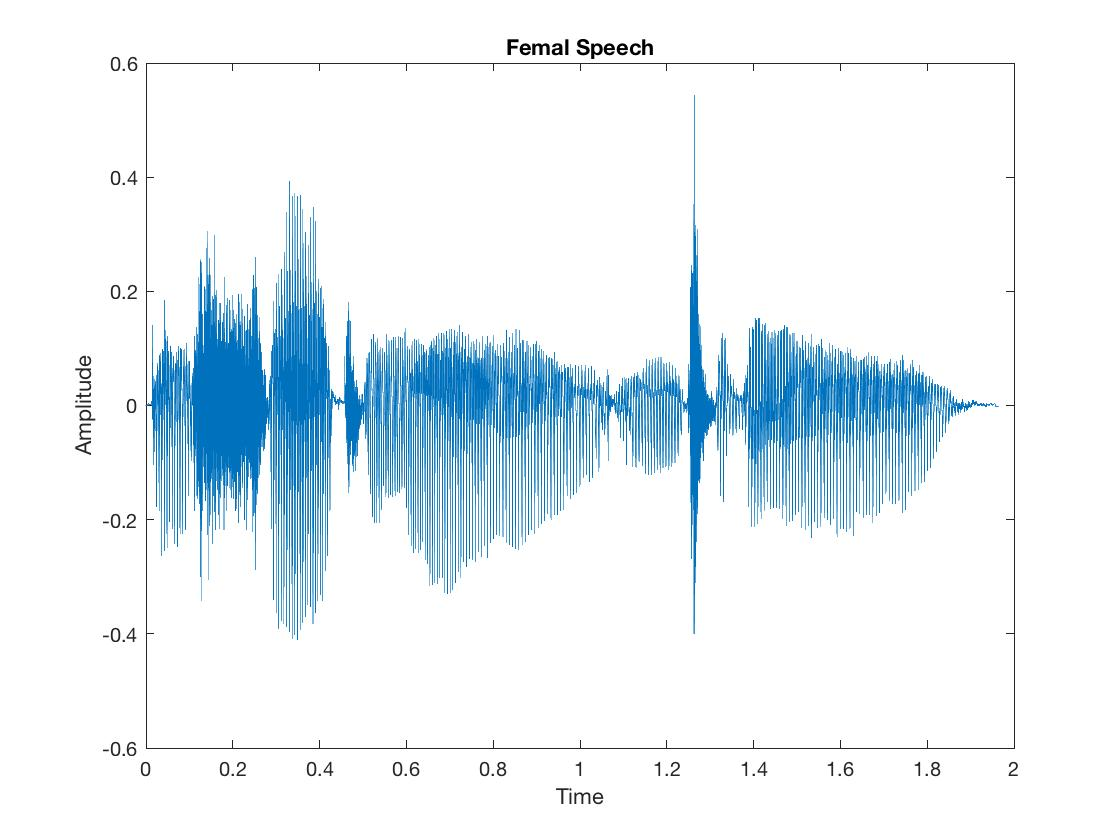
\includegraphics[width=0.75\textwidth]{female_time.jpg}
        \end{center}
        \caption{Female signal plot over time}

    \end{figure}
    The voiced sections of the signal can be locate on the plot where the oscillatory with some sort of pattern
    \begin{figure}[H]
        \begin{center}
            \leavevmode
            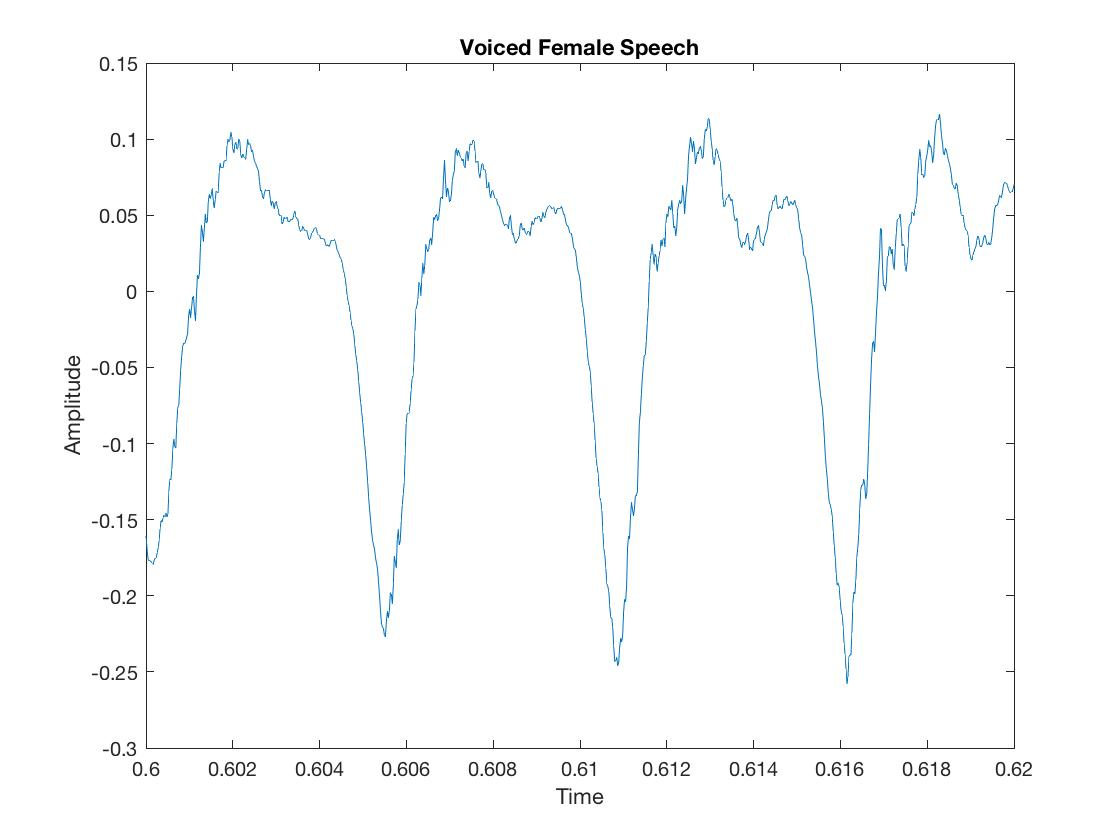
\includegraphics[width=0.75\textwidth]{voiced_time.jpg}
        \end{center}
        \caption{Voiced section of the female speech over time}
        \label{euler:1}
    \end{figure}
    The unvoiced section of the signal can be locate on the plot where the oscillatory without any sort of pattern
    \begin{figure}[H]
        \begin{center}
            \leavevmode
            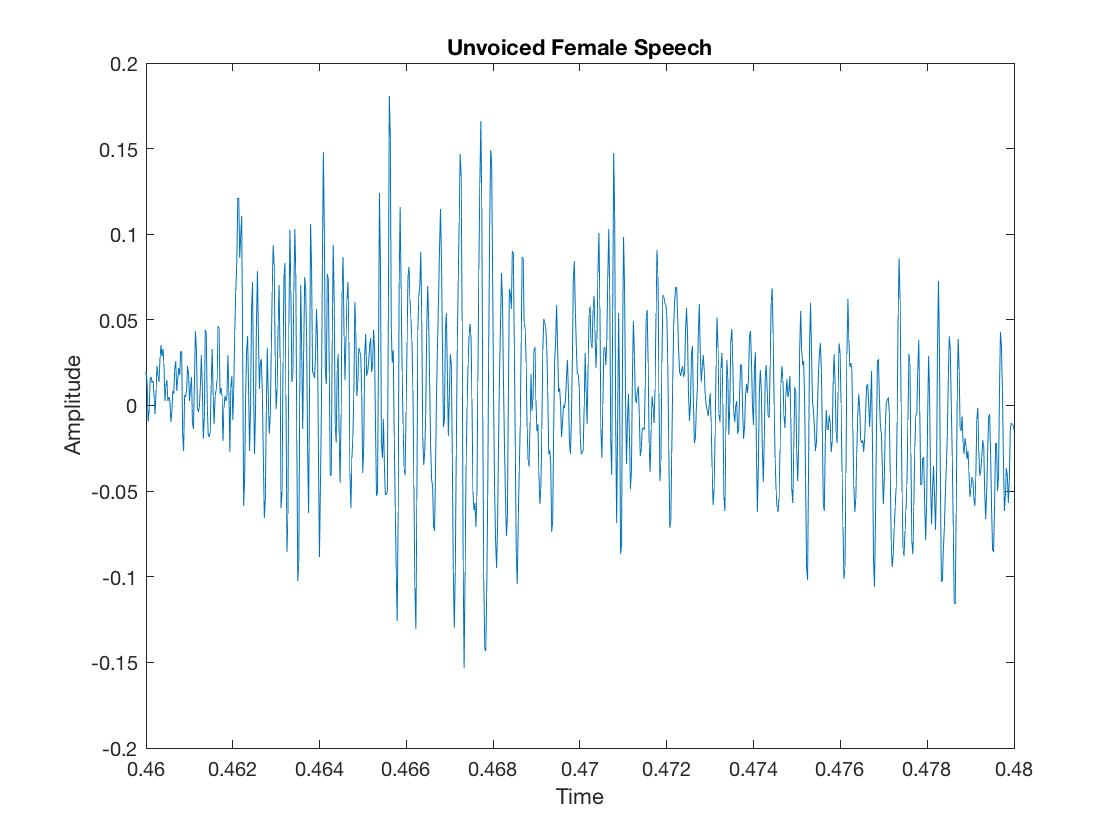
\includegraphics[width=0.75\textwidth]{unvoiced_time.jpg}
        \end{center}
        \caption{Unvoiced section of the female speech over time}
        \label{euler:1}
    \end{figure}
    \newpage
    \section{Spectrogram}
    For the music signal, the harmonic are highlighted on the plot the code generated the plot can be found at \texttt{spectplot.m}]
    \begin{figure}[H]
        \begin{center}
            \leavevmode
            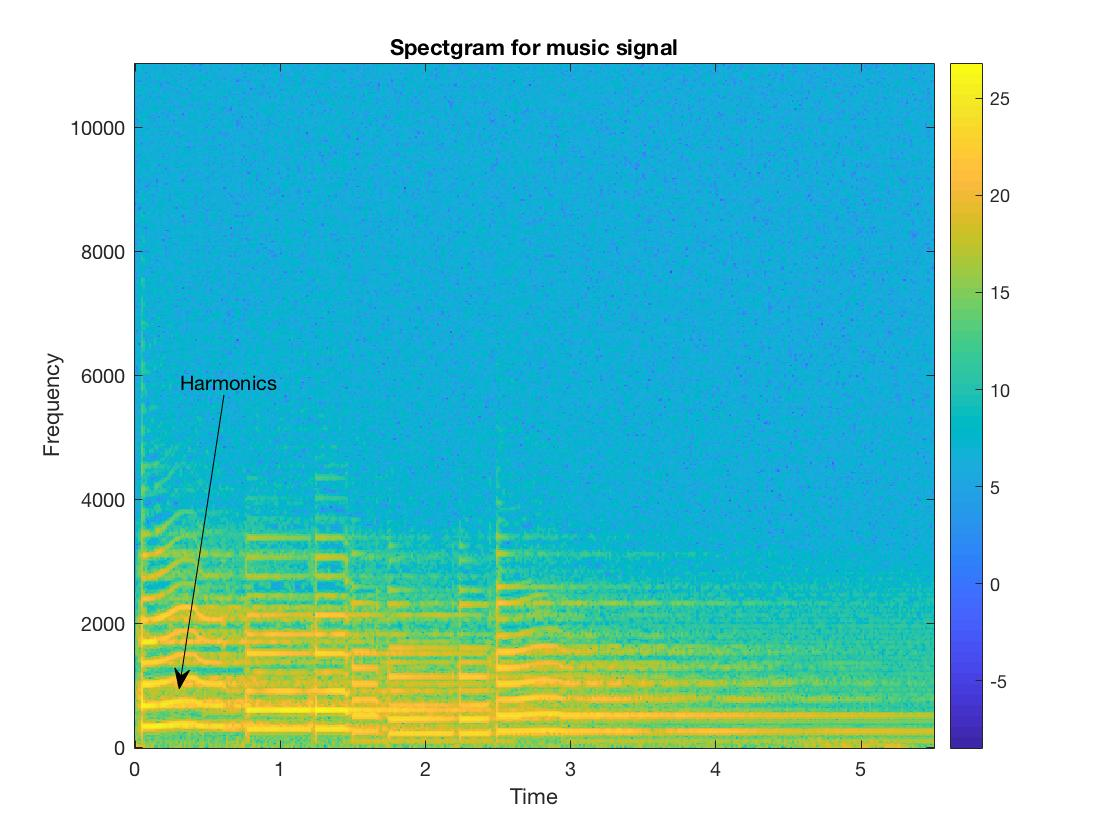
\includegraphics[width=0.5\textwidth]{spectgram_music.jpg}
        \end{center}
        \caption{Spectrogram for the music signal}
    \end{figure}
    For the female speech, it is possible to distinguish between voiced and unvoiced section from the plot, unvoiced section have no concentration on certain frequent;However, voiced section have an concentration on a certain frequency
    et. The voiced and unvoiced segment are highlighted on the diagram below
    \begin{figure}[H]
        \begin{center}
            \leavevmode
            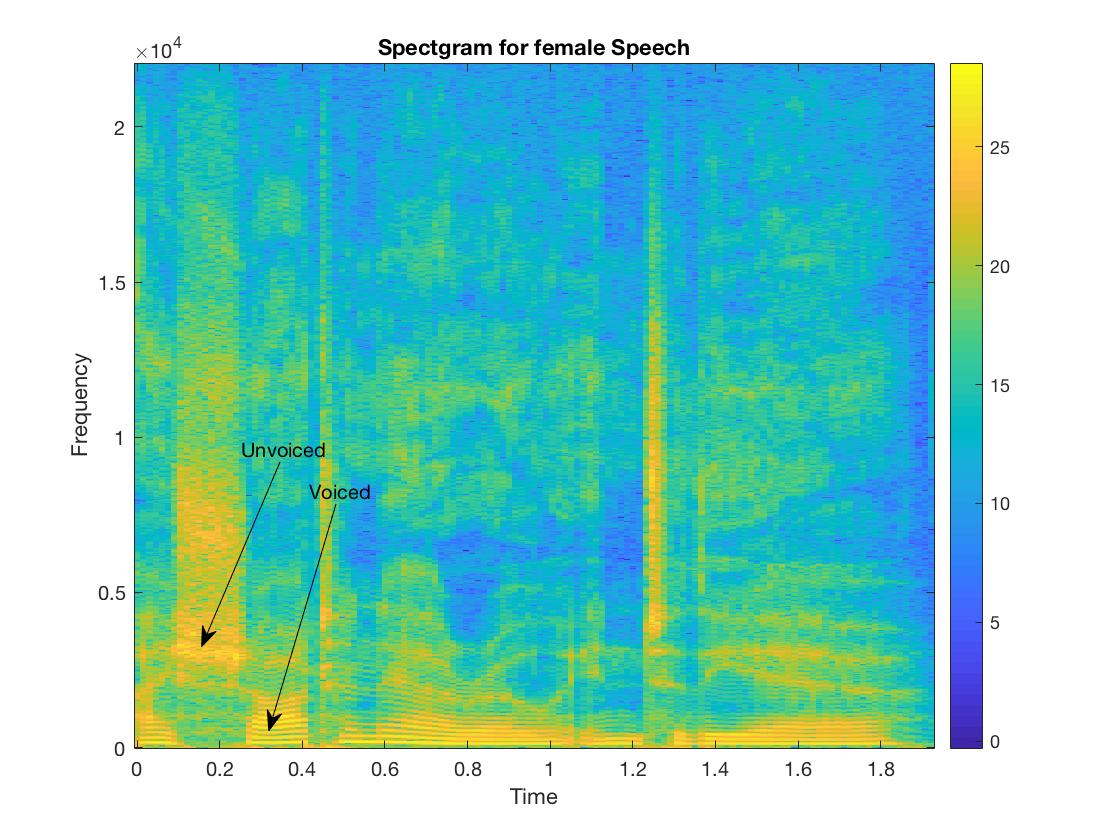
\includegraphics[width=0.65\textwidth]{spect_female.jpg}
        \end{center}
        \caption{Spectrogram for the female signal}
        \label{euler:1}
    \end{figure}
    \newpage
    \section{Cepstrogram}
    The plots below show the Spectrogram and Cepstrogram(normalized) for the music signal. the code for this section can be found at \texttt{ceptplot.m}
    \begin{figure}[H]
        \begin{center}
            \leavevmode
            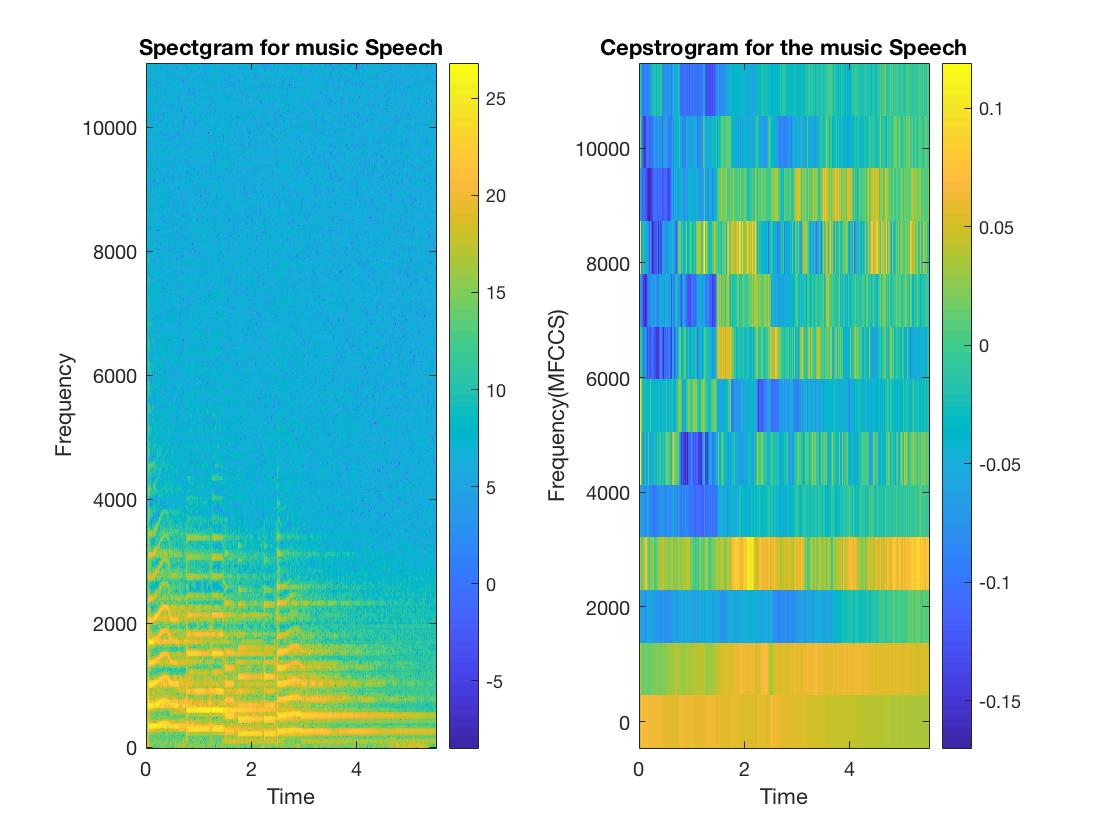
\includegraphics[width=0.5\textwidth]{cept_music.jpg}
        \end{center}
        \caption{Spectrogram for the female signal}
        \label{euler:1}
    \end{figure}
    Then, the cepstrogram of male and female speech samples are plotted together in order to compare them in the same phase
    \begin{figure}[H]
        \begin{center}
            \leavevmode
            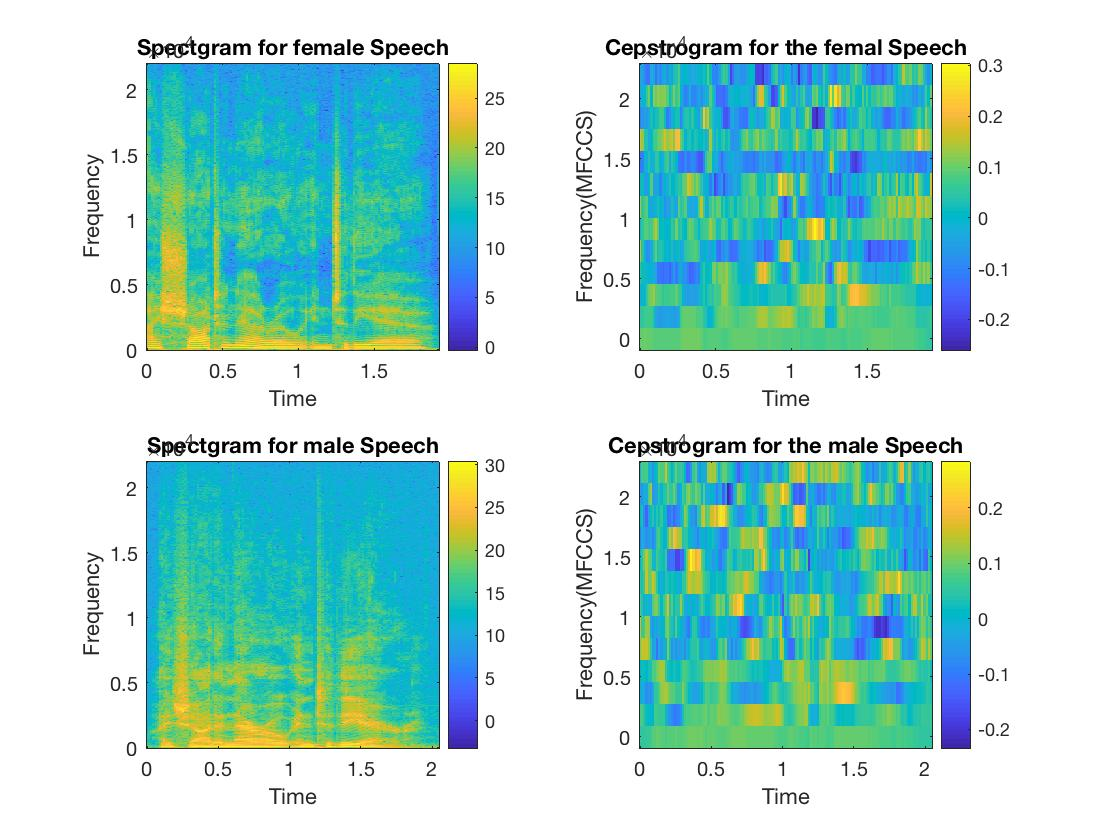
\includegraphics[width=0.75\textwidth]{cept_male_female.jpg}
        \end{center}
        \caption{Spectrogram for the female signal}
    \end{figure}
    \newpage
    \section{Correlation matrices}
    The following plot used the code \texttt{corr.m} to plot the correlation for the female speech sample
    \begin{figure}[H]
        \begin{center}
            \leavevmode
            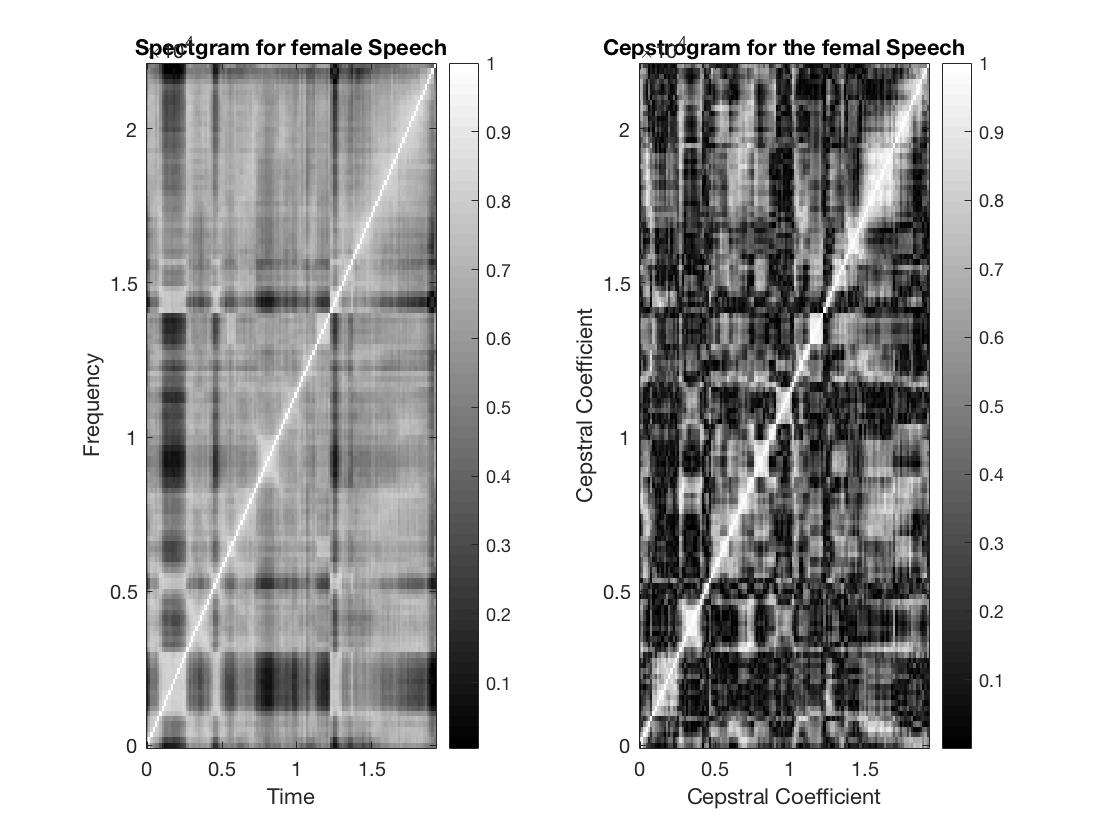
\includegraphics[width=0.75\textwidth]{corr.jpg}
        \end{center}
        \caption{Spectrogram for the female signal}
    \end{figure}
    \newpage
    \section{Questions}
    \begin{enumerate}[label=\alph*)]
        \item Which representation do you think is the easiest for you, as a human, to interpret, and why?
        \begin{adjustwidth}{2em}{0pt}
            In my opinion,the Spectrogram is much easier for me to interpret. Since it has a very clear reflection on the signal.
            the Spectrogram give a trend of the signal. It also very easy to distinguish between voiced and unvoiced sections
        \end{adjustwidth}
        \item Can you see that they represent the same phrase? Could a computer discover this? Why/why not?
        \begin{adjustwidth}{2em}{0pt}
            Even though male and female have different ascents and frequent range. It is still
            possible for human to recognize that they are represent the same phrase since there are many
            similarity between them such as the trends and the concentration on certain frequency. \\
            However, I don't think a computer can make the decision that those two Spectrogram represent the
            same phrase since the different in one region is too small for a computer to recognize
            them as a same phrase
        \end{adjustwidth}
        \item Can you see that they represent the same phrase now? What about a computer?
        \begin{adjustwidth}{2em}{0pt}
            It's almost impossible for me to distinguish those to cepstrogram since it's harder for me
            to find a similar pattern between them. However, I think it would be easier for computer to
            recognize that they are represent the same phrase since the cepstrogram divided near information
            into chunks which make it easier for computer to make a decision
        \end{adjustwidth}
        \item Which matrix, spectral or cepstral, looks the most diagonal to you?
        \begin{adjustwidth}{2em}{0pt}
            The cepstrogram looks more diagonal to me since its pattern are more clear to follow
        \end{adjustwidth}
    \end{enumerate}
    \section{Some thoughts on the possibility of confusing the MFCC representation}
    Can you think of a case where two utterances have noticeable differences to a human
    listener, and may come with different interpretations or connotations but still have very similar MFCCs\\
    \begin{adjustwidth}{2em}{0pt}
        The MFCC first translate the wave into spectral envelope field. which make us lose lots of
        information about the pitch. in such case, MFCC has trouble when analysis a same word with
        different pitch. for example, "I am scared" has a different with "I am scared?"
    \end{adjustwidth}
    What about the opposite situation: are there two signals that sound very similar to human, but have substantially
    different MFccs;
    \begin{adjustwidth}{2em}{0pt}
        cepstrogram analysis have divide the sound signal into
        low and high frequency domain, so that when a sound contain both low
        and high frequency signal(Which sound very noise to human). MFCCs can
        easier distinguish between them.
    \end{adjustwidth}
    \bibliography{references}
    \end{document}

